\chapter{Introduction}
\label{chapterlabel1}

    \section{Context} 

    The complex nature of human mobility has undergone a notable transformation in recent times due to various factors. Contemporary transportation has evolved, encompassing a dynamic interplay between private vehicles and public transport systems. This evolution has been further driven by the surging urban population, which has led to a paradigm shift in mobility patterns\citep{battyInventingFutureCities2018,townsendSmartCitiesBig2013}. Notably, the convergence of computational techniques, advanced data collection methods, and the utilisation of Artificial Intelligence (AI) has paved the way for innovative approaches to address the challenges posed by the new dynamic of human mobility. 
    
    Within this context, the study of human mobility has gained significant attention, focusing on multifaceted aspects such as city migration, rural depopulation, urban mobility pattern modelling, city population estimation, disaster-induced migration, climate-driven shifts, and predicting traffic dynamics and crowd movements. These areas emphasise mobility's dynamic and complex nature, reproducing the increasing complexity of contemporary human movement(\citep{battySizeScaleShape2008, lucaSurveyDeepLearning2021}. \cite{siminiDeepGravityModel2021} emphasise the expanding sphere of influence that human mobility acts on in many domains, from urban planning to epidemiology.
        
    The importance of human mobility modelling resonates deeply within various research domains, shaping our understanding of diverse processes. The shift in the dynamic of mobility flows impacted the spatial distribution, city density, population distribution, and disease dissemination. Such transformative impacts illustrate the role of mobility in shaping urban dynamics and social phenomena, in addition to the emergence of new computational tools to deal with this new scenario\citep{siminiDeepGravityModel2021, lucaSurveyDeepLearning2021}. 
    
    Mobility flows are complex, and people have various reasons for their travels, such as going to their jobs or schools. These routines usually happen on weekdays, creating a clear pattern that we can represent with a linear relationship with people's origin and destination flows\citep{siminiDeepGravityModel2021}. This basic understanding of daily urban movement allows us to see how people's travels impact public infrastructure, transportation options, and where people live and work.
    
    However, as seen in \ref{fig: context}, not all travel fits this pattern. The citizens also commute for leisure, sports, healthcare, and other reasons that do not follow a predictable schedule. These kinds of trips have a complex point A to point B and a point C, mostly without a daily pattern. We need different tools to handle the irregularity to grasp these more complex movements. One promising tool is neural networking, which can better comprehend and predict these intricate movements with a non-linear relationship analysis\citep{camburuExplainingDeepNeural2021}. As cities expand and people travel for various purposes, adopting these new methods can benefit designing transportation systems that capture diverse needs more effectively.
   
    \begin{figure}[H]
        \centering
        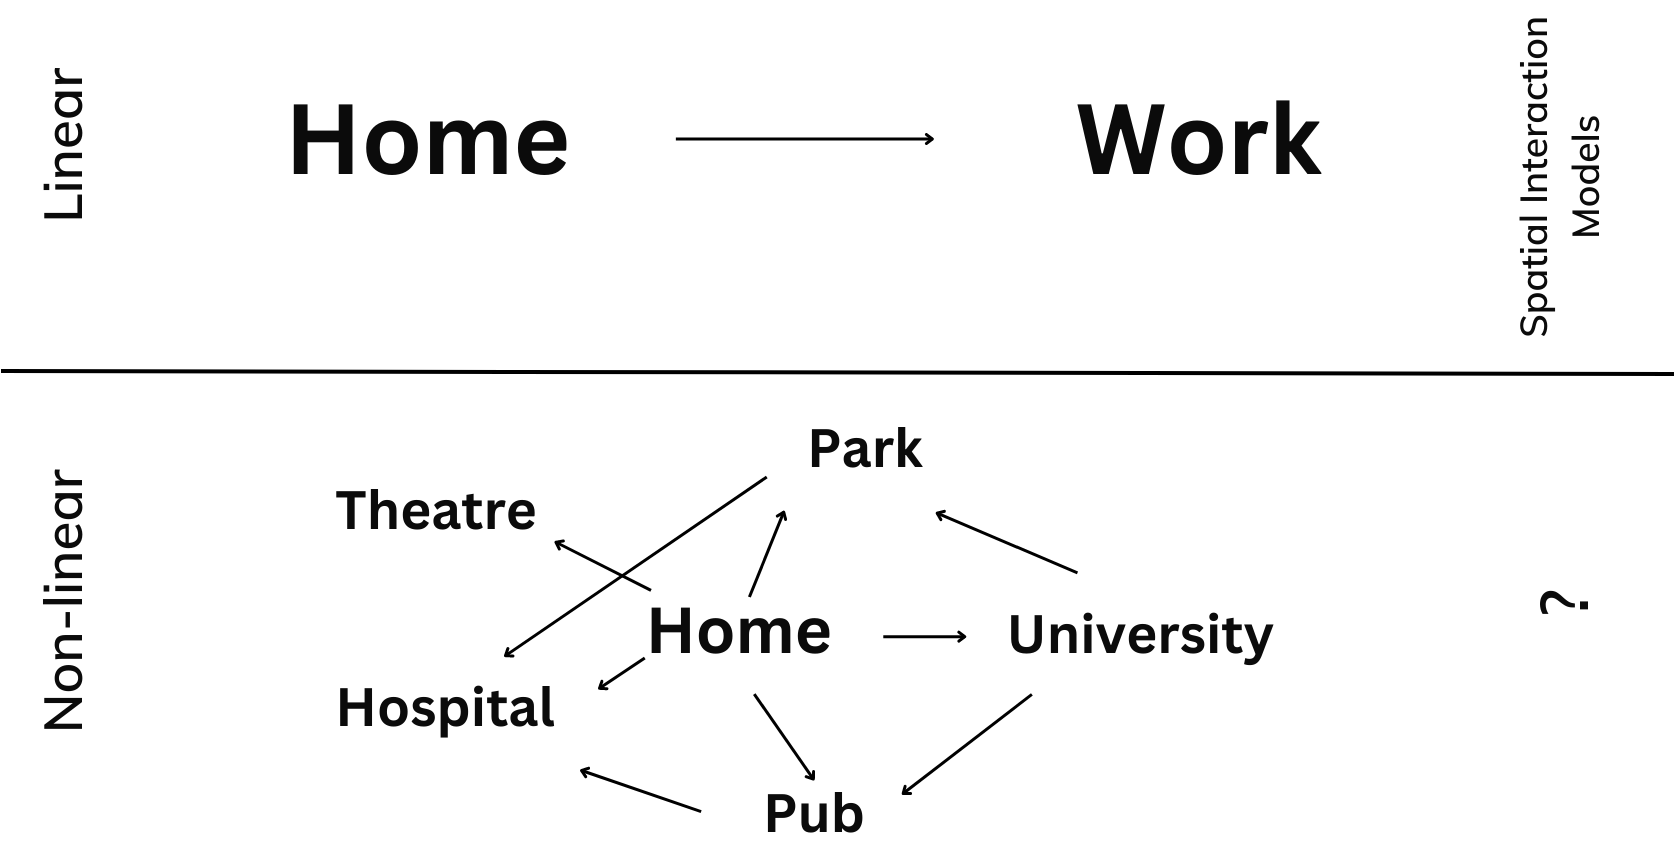
\includegraphics[width=12cm]{Images/context.png}
        \caption{Work x non-work flows}
        \label{fig: context}
    \end{figure}

   Using a spatial interaction model to predict movement patterns has proven to be a valuable tool for urban planning and understanding how cities change\citep{wilsonFamilySpatialInteraction1971b}. However, the rise of big data in today's technology-driven age, with access to vast amounts of previously unseen information, has posed challenges for traditional models. Therefore, new models such as the Deep Gravity Model, in which the Gravity Model is combined with neural network architecture, show great promise in efficiently estimating mobility flows. As a result, innovative approaches that involve artificial intelligence and machine learning are being explored to update transportation modelling methods. These modern methods hold great potential for revolutionising the way we model and plan for transportation in cities.

    In summary, urban mobility is a multifaceted challenge. Regular commuting forms a predictable pattern, but other types of travel involve diverse motivations and schedules. By embracing innovative techniques, we can unravel the complexities of various movements within cities. This adaptable approach to understanding mobility enhances our planning and accommodates the evolving dynamics of urban life and travel.
    
    Hence, the main objective of this study is to assess the effectiveness of the deep gravity model in predicting mobility patterns for non-work-related flows. In this regard, evaluating the Deep Gravity model's performance against traditional Spatial Interaction Models assumes significant importance. 

    This comparison between work-related and non-work-related flows offers a comprehensive understanding of the model's capabilities in estimating complex mobility patterns. Such an analysis is crucial in investigating the potential value that deep learning methodologies bring to non-work-related flow prediction and estimation.


    \section{Research Question}    

    How do Deep Gravity and Spatial Interaction Models differ in their predictive capabilities for estimating mobility flows, considering non-work-related and work-related trips?

   

    \section{Report Structure}

    \begin{itemize}
        \item \textbf{Chapter 2:} Literature Review - This chapter overviews key methodologies and limitations in estimating mobility flows. It delves into the structure of the spatial interaction model while introducing the application of deep learning to mobility flow analysis. Additionally, the chapter introduces the deep gravity model as another method for flow estimation. 
        \item \textbf{Chapter 3:} Methodology - This chapter explains the architectural foundations of both models. It also delves into the dataset employed in this study and how it was structured for utilisation in both models. The chapter concludes by outlining the evaluation metrics that will be used to assess the performance of these models.
        \item \textbf{Chapter 4:} Results and Discussion - First, the evaluation of the models takes centre stage. The chapter showcases visualisations of the generated flows and presents the principal findings alongside their associated limitations.
        \item \textbf{Chapter 5:} Conclusion - The concluding chapter summarises the significance of the analysis undertaken. It also underscores potential avenues for further investigation in the following studies.  
    \end{itemize}




% Some stuff about things.\cite{example-citation} Some more things. 

% Inline citation: \bibentry{example-citation}

